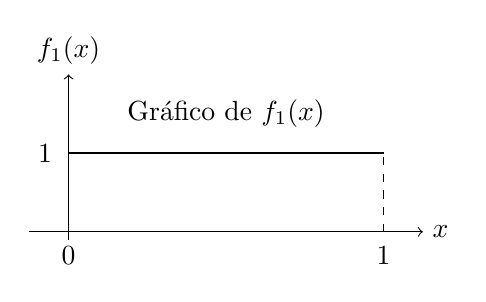
\begin{tikzpicture}
    % Draw x and y axes
    \draw[->] (-0.5, 0) -- (4.5, 0) node[right] {$x$};
    \draw[->] (0, -0.1) -- (0, 2) node[above] {$f_1(x)$};
    
    % Draw the function f_1
    \draw[thick] (0, 1) -- (4, 1); % f_1 is 1 in [0,1]
    %\draw[dashed] (0, 0) -- (4, 0); % Dashed line at y = 0
    
    % Vertical lines to close the graph at 0 and 1
    %\draw[thick] (0, 0) -- (0, 1);
    \draw[dashed] (4, 0) -- (4, 1);
    
    % Labels for the intervals and function values
    \node at (4,-0.3) {$1$};
    \node at (0,-0.3) {$0$};
    \node at (-0.3,1) {$1$};

    % Add title
    \node at (2, 1.5) {Gráfico de $f_1(x)$};
    
\end{tikzpicture}

\begin{minipage}{0.45\textwidth}
    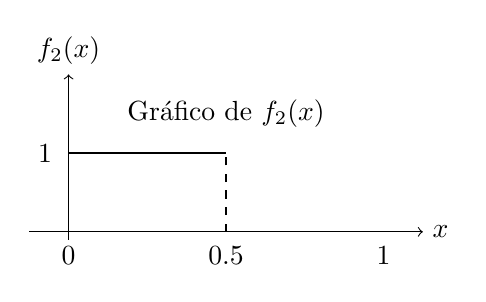
\begin{tikzpicture}
        % Draw x and y axes
        \draw[->] (-0.5, 0) -- (4.5, 0) node[right] {$x$};
        \draw[->] (0, -0.1) -- (0, 2) node[above] {$f_2(x)$};
        
        % Draw the function f_2
        \draw[thick] (0, 1) -- (2, 1); % f_2 is 1 in [0,0.5]
        \draw[dashed] (2, 0) -- (2, 1);
        
        % Labels for the intervals and function values
        \node at (4,-0.3) {$1$};
        \node at (2,-0.3) {$0.5$};
        \node at (0,-0.3) {$0$};
        \node at (-0.3,1) {$1$};
    
        % Add title
        \node at (2, 1.5) {Gráfico de $f_2(x)$};
    \end{tikzpicture}
\end{minipage}
\begin{minipage}{0.45\textwidth}
    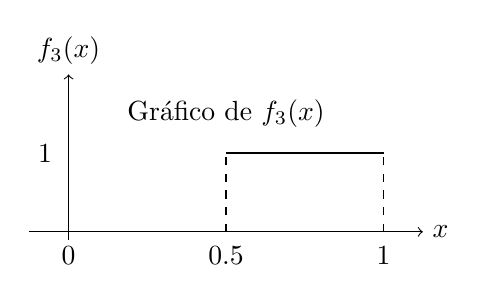
\begin{tikzpicture}
        % Draw x and y axes
        \draw[->] (-0.5, 0) -- (4.5, 0) node[right] {$x$};
        \draw[->] (0, -0.1) -- (0, 2) node[above] {$f_3(x)$};
        
        % Draw the function f_3
        \draw[thick] (2, 1) -- (4, 1); % f_3 is 1 in [0.5,1]
        \draw[dashed] (4, 0) -- (4, 1);
        \draw[dashed] (2, 0) -- (2, 1);
        
        % Labels for the intervals and function values
        \node at (4,-0.3) {$1$};
        \node at (2,-0.3) {$0.5$};
        \node at (0,-0.3) {$0$};
        \node at (-0.3,1) {$1$};
    
        % Add title
        \node at (2, 1.5) {Gráfico de $f_3(x)$};
    \end{tikzpicture}
\end{minipage}

\begin{minipage}{0.24\textwidth}
    \begin{tikzpicture}
        % Draw x and y axes
        \draw[->] (-0.25, 0) -- (2.25, 0) node[right] {$x$};
        \draw[->] (0, -0.1) -- (0, 2) node[above] {$f_4(x)$};
        
        % Draw the function f_4
        \draw[thick] (0, 1) -- (0.5, 1); % f_4 is 1 in [0,0.25]
        \draw[dashed] (0.5, 0) -- (0.5, 1);
        
        % Labels for the intervals and function values
        \node at (2,-0.3) {$1$};
        \node at (0,-0.3) {$0$};
        \node at (-0.3,1) {$1$};
    \end{tikzpicture}
\end{minipage}
\begin{minipage}{0.24\textwidth}
    \begin{tikzpicture}
        % Draw x and y axes
        \draw[->] (-0.25, 0) -- (2.25, 0) node[right] {$x$};
        \draw[->] (0, -0.1) -- (0, 2) node[above] {$f_5(x)$};
        
        % Draw the function f_5
        \draw[thick] (0.5, 1) -- (1, 1); % f_5 is 1 in [0.25,0.5]
        \draw[dashed] (0.5, 0) -- (0.5, 1);
        \draw[dashed] (1, 0) -- (1, 1);
        
        % Labels for the intervals and function values
        \node at (2,-0.3) {$1$};
        \node at (0,-0.3) {$0$};
        \node at (-0.3,1) {$1$};
    \end{tikzpicture}
\end{minipage}
\begin{minipage}{0.24\textwidth}
    \begin{tikzpicture}
        % Draw x and y axes
        \draw[->] (-0.25, 0) -- (2.25, 0) node[right] {$x$};
        \draw[->] (0, -0.1) -- (0, 2) node[above] {$f_6(x)$};
        
        % Draw the function f_6
        \draw[thick] (1, 1) -- (1.5, 1); % f_6 is 1 in [0.5,0.75]
        \draw[dashed] (1, 0) -- (1, 1);
        \draw[dashed] (1.5, 0) -- (1.5, 1);
        
        % Labels for the intervals and function values
        \node at (2,-0.3) {$1$};
        \node at (0,-0.3) {$0$};
        \node at (-0.3,1) {$1$};
    \end{tikzpicture}
\end{minipage}
\begin{minipage}{0.24\textwidth}
    \begin{tikzpicture}
        % Draw x and y axes
        \draw[->] (-0.25, 0) -- (2.25, 0) node[right] {$x$};
        \draw[->] (0, -0.1) -- (0, 2) node[above] {$f_7(x)$};
        
        % Draw the function f_7
        \draw[thick] (1.5, 1) -- (2, 1); % f_7 is 1 in [0.75,1]
        \draw[dashed] (1.5, 0) -- (1.5, 1);
        \draw[dashed] (2, 0) -- (2, 1);
        
        % Labels for the intervals and function values
        \node at (2,-0.3) {$1$};
        \node at (0,-0.3) {$0$};
        \node at (-0.3,1) {$1$};
    \end{tikzpicture}
\end{minipage}